\section{实验}

我们在三种实际的智能体训练场景中评估 Agent Lightning v1.0：搜索、通用指令遵循与编程。我们沿用 Search-R1~\cite{searchr1} 的实验设置训练搜索智能体，沿用 LLM-in-Sandbox~\cite{llminsandbox} 的设置训练通用指令遵循智能体。对编程智能体，我们从 SWE-smith~\cite{swesmith} 构建训练数据。

我们发现现有框架很少提供完整、可复现的编程智能体训练示例，可能源于数据清洗复杂、环境搭建困难与所需算力巨大。因此我们聚焦编程智能体，详细描述其训练过程，目标是提供一个完整可复现、仅需适量资源的示例。

\subsection{搜索智能体}

我们沿用 Search-R1~\cite{searchr1} 的实验设置，训练一个将推理与搜索引擎查询交织、利用检索到的段落回答知识密集问题的搜索智能体。策略模型为 Llama-3.2-3B-Instruct~\cite{llama3}，用 GRPO~\cite{deepseekmath} 优化。在 HotpotQA~\cite{hotpotqa} 训练集上训练。评估时，从 HotpotQA、2WikiMultiHopQA~\cite{2wikimultihopqa}、MuSiQue~\cite{musique}、Bamboogle~\cite{bamboogle}、TriviaQA~\cite{triviaqa} 与 Natural Questions~\cite{naturalquestions} 各采样 50 个样本。训练批次大小 512，每个 prompt 采样 4 次 rollout，每 10 个训练步评估一次。奖励指标为精确匹配（EM）。

图~\ref{fig:search-r1-training} 总结了训练动态。平均训练奖励稳步上升。验证集奖励从 25.1\% 提升至 41.7\%，绝对提升 16.6\%。

\begin{figure}[t]
  \centering
  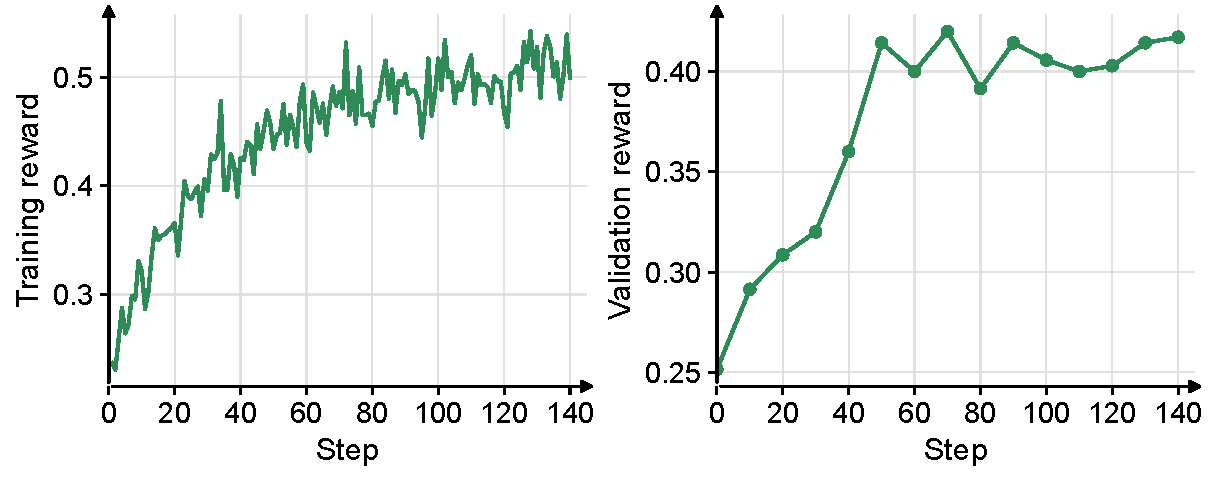
\includegraphics[width=0.65\textwidth]{figures/search-r1-metrics.pdf}
  \caption{搜索智能体训练动态。从左到右：平均训练奖励与平均验证奖励。}
  \label{fig:search-r1-training}
\end{figure}

\subsection{通用指令遵循智能体}

我们沿用 LLM-in-Sandbox~\cite{llminsandbox} 的实验设置训练通用指令遵循智能体。该智能体通过计算机沙箱访问外部资源、管理文件并执行代码，解决多样化的非编程任务。使用原作者提供的智能体脚手架。策略模型为 Qwen3-4B-Instruct-2507~\cite{qwen3}，用 RLOO~\cite{rloo} 优化。使用 Instruction Pre-Training~\cite{instructionpretraining} 发布的数据集，按 80\%/20\% 划分训练与评估。训练批次大小 8，每个 prompt 采样 8 次 rollout，每 20 个训练步评估一次。

图~\ref{fig:llm-in-sandbox-training} 显示批次级训练奖励噪声较大，而验证奖励呈现清晰的上升趋势：从 51.9\% 提升至 70.2\%，绝对提升 18.3\%。

\begin{figure}[t]
  \centering
  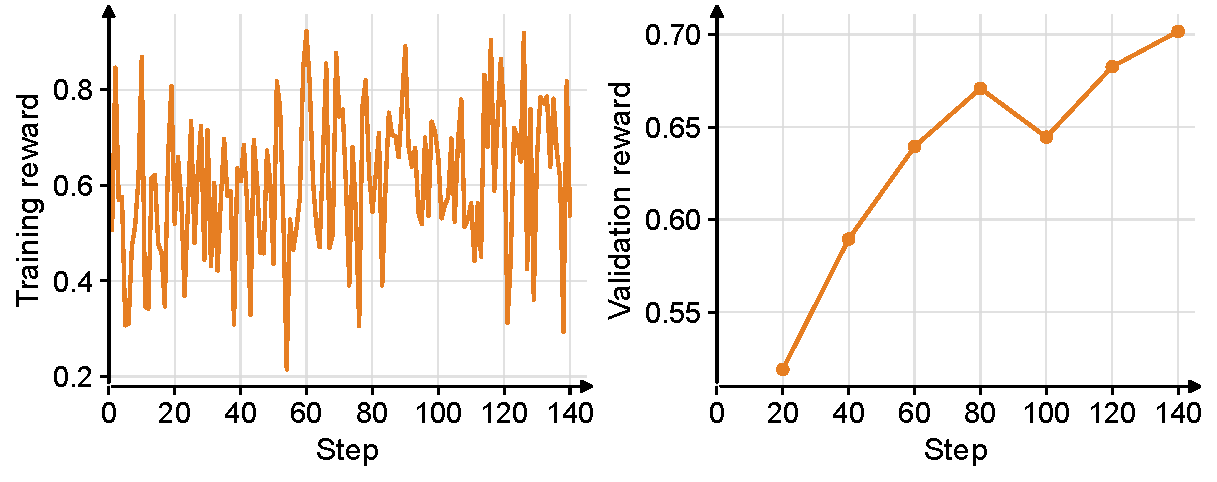
\includegraphics[width=0.65\textwidth]{figures/llm-in-sandbox-metrics.pdf}
  \caption{通用指令遵循智能体训练动态。从左到右：平均训练奖励与平均验证奖励。}
  \label{fig:llm-in-sandbox-training}
\end{figure}

\subsection{编程智能体}

我们基于 Qwen3.5-9B~\cite{qwen35}，使用 SWE-smith 数据集~\cite{swesmith} 派生的任务训练编程智能体。使用 mini-SWE-agent~\cite{minisweagent} 作为智能体脚手架，与仓库环境交互、执行命令并产出代码修改。为获得可靠的训练信号，我们应用详细的数据过滤管线，引入防奖励黑客保护措施，并实现健壮编程智能体训练所需的额外措施。下面描述这些实现细节。

\subsubsection{数据集预处理与过滤}

SWE-smith 是一个大规模可执行软件工程任务数据集，通过向真实 Python 仓库引入 bug 构建而成。它包含来自 128 个仓库的 59,136 个任务，附问题陈述、代码补丁与验证解法的测试~\cite{swesmith}。其 Docker 镜像仅占 295~GB~\cite{swesmith}，远小于 R2E-Gym~\cite{r2egym} 所需的 4~TB 与 SWE-Gym~\cite{swegym} 所需的 6~TB。

对每个任务，SWE-smith 先将仓库切换到对应问题分支，要求编程智能体修改代码库，然后运行任务专属测试套件判断提交的修改是否解决问题。

我们在发布数据中发现以下问题：
\begin{itemize}
  \item 59,136 条记录中有 18,033 条问题陈述为空。
  \item 1,265 条记录对应的问题分支在所提供 Docker 镜像中缺失。
  \item 部分任务需要大规模测试套件。例如 \texttt{python-jsonschema} 需要执行 7,000 多个测试，消耗大量 CPU 与内存。
\end{itemize}

因此我们移除问题陈述为空、问题分支缺失或测试数超过 200 的任务。剩余任务的难度分布仍然高度偏斜、训练信号有限，因此我们额外应用基于模型的难度过滤：对每个候选任务用 Qwen3.5-9B 运行四次——四次 rollout 全部解决的任务被移除，成功与失败并存的任务被保留，得到约 5,000 个样本。为避免结果集过于简单，我们额外采样 1,000 个四次 rollout 全部失败的任务。最终划分包含约 6,000 个训练样本与 400 个测试样本。

\subsubsection{防止奖励黑客}
\label{subsec:reward-hacking}

训练期间，我们观察到若干奖励黑客行为——智能体绕过预期的解题过程直接获取参考源代码：
\begin{enumerate}
  \item 使用 Git 历史定位正确提交。
  \item 使用 \texttt{wget} 或 \texttt{curl} 从 GitHub 获取上游源代码。
  \item 使用 \texttt{pip} 下载软件包源代码。
  \item 使用 Python 网络库（如 \texttt{urllib}）下载源代码。
\end{enumerate}

我们引入两道防护。第一，禁用 Git 命令并向智能体隐藏 \texttt{.git} 目录，阻止其检查提交历史。第二，强制 Kubernetes 网络策略，阻断一般出站网络访问，只允许连接显式白名单服务。两项措施共同要求智能体仅凭问题陈述与本地信息解题。

\subsubsection{训练动态}

\begin{figure}[t]
  \centering
  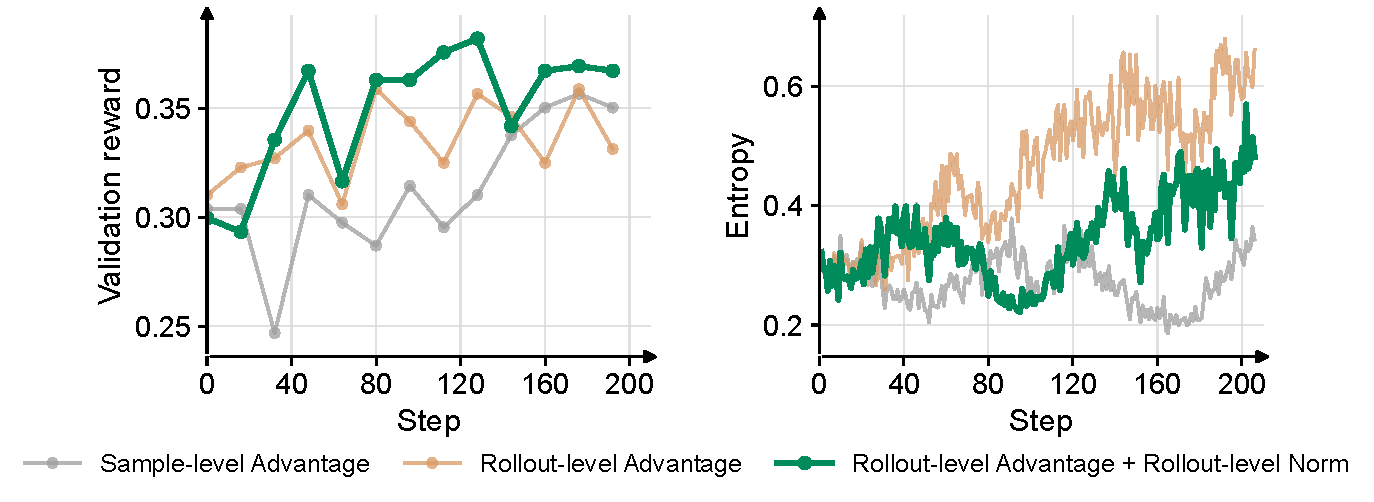
\includegraphics[width=0.75\textwidth]{figures/smith-ablation-metrics.pdf}
  \caption{样本级优势、rollout 级优势与 rollout 级优势 + rollout 级归一化三种设置的编程智能体训练动态。左：验证奖励。右：策略熵。}
  \label{fig:smith-ablation-training}
\end{figure}

\begin{figure}[t]
  \centering
  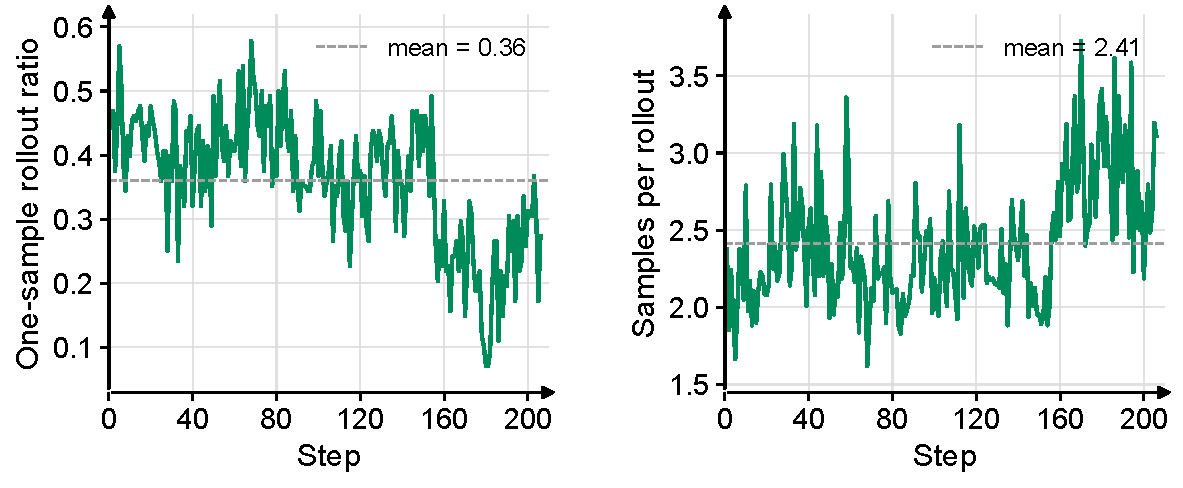
\includegraphics[width=0.75\textwidth]{figures/smith-merge-sample-metrics.pdf}
  \caption{rollout 级优势 + rollout 级归一化训练的 rollout 合并行为。左：恰好产生一个训练样本的 rollout 占比。右：每次 rollout 产生的平均训练样本数。虚线标记训练全程均值。}
  \label{fig:smith-merge-sample-metrics}
\end{figure}


如第~\ref{sec:challenges} 节所述，由于一次 rollout 的样本数常由重分词等偶然因素驱动，优势计算（第~\ref{subsec:advantage-calculation} 节）与损失归一化（第~\ref{subsec:loss-normalization} 节）都应在 rollout 层面而非样本层面计算。我们在编程智能体训练中对比三种设置验证这一设计选择，三者均使用相同的底层 GRPO 目标：
\begin{itemize}
  \item \emph{样本级优势}：样本级优势 + 式~\ref{eq:token-mean} 的 token 均值损失；
  \item \emph{rollout 级优势}：仅将优势计算切换到 rollout 级，保留 token 均值损失；
  \item \emph{rollout 级优势 + rollout 级归一化}：进一步将 token 均值损失替换为式~\ref{eq:rollout-mean} 的 rollout 级 token 均值损失。
\end{itemize}
图~\ref{fig:smith-ablation-training} 对比三种设置。最后一种变体获得最高的验证奖励：第 128 步达到 38.2\%，相比之下基线为 35.0\%，仅修复 rollout 优势时为 33.1\%。其策略熵增长也更慢、训练全程比仅修复 rollout 优势的变体更稳定。这些结果表明，损失归一化在提升验证奖励的同时控制了修正后的 rollout 优势带来的熵增。我们还在 SWE-bench Verified~\cite{swebench} 上评估了 rollout 级优势 + rollout 级归一化检查点：第 208 步从 41.8\% 提升至 56.4\%。由于编程智能体轨迹长度差异很大，rollout 级优势变体会尽可能将轨迹合并为训练行以减少填充浪费，由此产生动态的每-rollout 训练样本数：平均仅 36\% 的 rollout 保持为单一完全合并行，每次 rollout 平均产生 2.41 个训练样本（图~\ref{fig:smith-merge-sample-metrics}）。
